\documentclass[letter, 10pts]{article}
\usepackage[monocolor]{../math232/ahsansabit}
\usepackage[]{float}
\usepackage{tikz}
\usepackage{tikz-3dplot}
\usepackage[outline]{contour} % glow around text
\usepackage{xcolor}
\usepackage{pdfpages}
\usepackage{physics}
\usepackage{multicol}
\title{Solid State Physics : : Homework 03}
\author{Ahmed Saad Sabit, Rice University}
\date{\today}
\newcommand{\hb}{\hbar}
\newcommand{\U}{\uparrow}
\newcommand{\D}{\downarrow}
\usepackage[]{hyperref}
\usepackage[]{braket}
\usepackage[]{pdfpages}
\begin{document}
\maketitle

\section*{Problem 01} 
\subsection*{(a)} 
\hrule
\[
	B = \frac{\hb }{e l_B^2} = 5048.51 \, T 
\] 

\subsection*{(b)} 
\hrule 
\[
\omega_c = \frac{eB}{m} \to \hb \omega_c \sim k_B T \implies B  \sim \frac{k_B T m}{\hb e} 
\]
\[
B \sim 15.7 \, T
\] 

\subsection*{(c)} 
\hrule
Small Effective mass and Large Magnetic field means 
\[
\frac{eB}{m} \gg 1 
\]
So now our resistivity tensor can approximately behave like 
\[
	\rho \sim \rho_0 \begin{bmatrix} 0 & \omega_c \tau \\ - \omega_c \tau & 0 \end{bmatrix} 
\]
It's quite obvious to see that a current $\begin{bmatrix} j \\ 0 \end{bmatrix} $ would be caused by electric field along 
\[
	E_{1,0}   = \rho  \vec{j}  \sim \rho_0 \begin{bmatrix} 0 & \omega_c \tau \\ - \omega_c \tau & 0 \end{bmatrix}  \begin{bmatrix} j \\ 0 \end{bmatrix}  =  \begin{bmatrix} 0 \\ - \rho_0 j \omega_c \tau \end{bmatrix} 
\] 
Similarly for a current along $\begin{bmatrix} 0 \\ j \end{bmatrix} $ we have 
\[
	E_{0,1} \sim \begin{bmatrix} \rho_0 j \omega_c \tau \\ 0  \end{bmatrix} 
\]
The current is ``mostly" \textbf{perpendicular} to the direction of Electric field.

\subsection*{(d)} 
\hrule 
\begin{itemize}
	\item Turn on the Magnetic field: now the carriers have a cyclotron frequency $ \omega_c$ were $m$ is the effective mass in $\omega_c = e B / m$. 
	\item Now let's try to measure the resistance as shown in the figure of the problem. That requires us to apply a voltage difference (as in the figure). For this, the electric field also happens to point in the direction along the voltage difference. 
	\item The current is also being measured \textbf{parallel} to the voltage difference as it can be seen in the figure. But from our analysis in (c) we just saw for \emph{high magnetic field} and \emph{low effective} mass where we can safely project the approximation $ B / m \gg 1$ then \emph{current flow is perpendicular to supplied electric field}. 
	\item So the amount of current flow \textbf{along} the electric field in this given system is extremely low (given how well our $B / m$ ratio is). This invokes a ``Magnetoresistance" (Tanner would be happy to hear this) which explains why the resistance goes up. 
\end{itemize}

\subsection*{Documented Calculator Assist}
\hrule 
\begin{figure}[htpb]
	\centering
	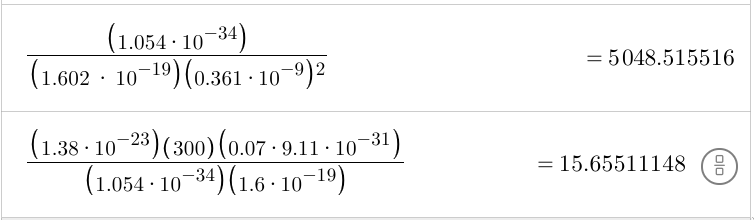
\includegraphics[width=0.8\textwidth]{./fig/3/2.png}
	\caption{./fig/3/1.png}
	\label{fig:-fig-3-1-png}
\end{figure}
\section*{Problem 02}
\hrule 
\subsection*{a	}
\renewcommand{\vec}{\mathbf}
\url{https://proofwiki.org/wiki/Curl_of_Vector_Cross_Product}
\begin{align*}
\vec{B} = \nabla \times  \vec{A} &= \nabla \times 
\left(\frac{1}{2} \vec{B} \times \vec{r} \right)\\
&=  
\left(\vec{r} \cdot  \nabla \right) \frac{1}{2}\vec{B} - 
\vec{r} \left(\nabla \cdot \frac{1}{2} \vec{B}\right) 
- (\frac{\vec{B}}{2} \cdot  \nabla ) \vec{r} + 
\frac{1}{2} \vec{B} \left(\nabla \cdot \vec{r}\right)
\\
&= 0 - 0 - \sum_{j=1}^{3} \left(
\sum_{n=1}^{3} \frac{B_n}{2} \frac{\partial r_j }{\partial x_n} \hat{x_j}
\right) 
+ \sum_{n=1}^{3} \frac{1}{2} \left(3 B_n \hat{x_n}\right) \\
&=- 
\sum_{n=1}^{3} \frac{B_n}{2}  \hat{x_n}
+ \sum_{n=1}^{3} \frac{1}{2} \left(3 B_n \hat{x_n}\right) \\
&=\frac{1}{2} 
\sum_{n=1}^{3} - {B_n}  \hat{x_n}
 +3 B_n \hat{x_n} \\
& = \sum_{n=1}^{3} B_n \hat{x}_n = \vec{B}
\end{align*}



\subsection*{(b)}
\hrule


\[
\mathcal{H} = \frac{(\mathbf{p} + e \mathbf{A})^2}{2m} + g\mu_B \mathbf{B} \cdot \sigma + V(r)
\]

Expanding \( (\mathbf{p} + e \mathbf{A})^2 \)

\[
(\mathbf{p} + e \mathbf{A})^2 = \mathbf{p}^2 + e (\mathbf{p} \cdot \mathbf{A} + \mathbf{A} \cdot \mathbf{p}) + e^2 \mathbf{A}^2
\]

\( \mathbf{A} \) is a function of position, so we can ignore order of dot product, 

\[
\mathbf{p} \cdot \mathbf{A} + \mathbf{A} \cdot \mathbf{p} = 2 \mathbf{p} \cdot \mathbf{A}
\]

Thus,

\[
\mathcal{H} = \frac{\mathbf{p}^2}{2m} + \frac{e}{2m} (\mathbf{p} \cdot \mathbf{A} + \mathbf{A} \cdot \mathbf{p}) + \frac{e^2}{2m} \mathbf{A}^2 + g\mu_B \mathbf{B} \cdot \sigma + V(r)
\]

\( \mathbf{A} = \frac{1}{2} \mathbf{B} \times \mathbf{r} \)
\[
\mathbf{p} \cdot \mathbf{A} = \mathbf{p} \cdot \left(\frac{1}{2} \mathbf{B} \times \mathbf{r} \right) = \frac{1}{2} \mathbf{B} \cdot (\mathbf{p} \times \mathbf{r})
\]

which gives:

\[
\mathcal{H} = \frac{\mathbf{p}^2}{2m} + \frac{e}{2m} \mathbf{p} \cdot (\mathbf{B} \times \mathbf{r}) + \frac{e^2}{2m} \left( \frac{1}{4} |\mathbf{B} \times \mathbf{r}|^2 \right) + g\mu_B \mathbf{B} \cdot \sigma + V(r)
\]


\subsection*{(c)}
\hrule
First of all we refer to a formula table and also use the vector identity from previous homework,
\[
\vec{p} \cdot  \left(\vec{B} \times \vec{r}\right) = (\vec{p} \times  \vec{r}) \cdot  \vec{B} = \vec{L} \cdot  \vec{B} 
\] 
This lets us rewrite
\[
\frac{e}{2m} \vec{p}\cdot \left(\vec{B} \times \vec{r}\right) = \frac{e}{2m} \vec{B} \cdot  \vec{L} 
\] 	
Using $\mu_B = e \hb / 2 m$ we solve
\[
\frac{e}{2m} \vec{B} \cdot \vec{L} = \mu_B \frac{\vec{B}\cdot \vec{L}}{\hb}
\] 
Substitute in what we had gotten, 


\[
\mathcal{H} = \frac{\mathbf{p}^2}{2m} + \frac{e}{2m} \mathbf{p} \cdot (\mathbf{B} \times \mathbf{r}) + \frac{e^2}{2m} \left( \frac{1}{4} |\mathbf{B} \times \mathbf{r}|^2 \right) + g\mu_B \mathbf{B} \cdot \sigma + V(r)
\]


\[
\mathcal{H} = \frac{\mathbf{p}^2}{2m} + \mu_B \frac{\vec{B}\cdot \vec{L}}{\hb} + \frac{e^2}{2m} \left( \frac{1}{4} |\mathbf{B} \times \mathbf{r}|^2 \right) + g\mu_B \mathbf{B} \cdot \sigma + V(r)
\]

\[\boxed{
\mathcal{H} = \frac{\mathbf{p}^2}{2m} + \mu_B \vec{B}\cdot
\left( \frac{\vec{L}}{{\hb}} + g \vec{\sigma} \right)+ \frac{e^2}{2m} \left( \frac{1}{4} |\mathbf{B} \times \mathbf{r}|^2 \right)+ V(r)
}\]

\subsection*{(d)}
\hrule
First of all 
\begin{align*}
	\vec{B} \times \vec{r} &= B \left(\hat{z}\right) \times  (x \hat{x}  +y \hat{y}  )
	\\
	&=-  B x \hat{y}- B y \hat{x} \\
	| \vec{B} \times  \vec{r} | ^2 &= B^2 (x^2  + y^2)
\end{align*}
For quantum mechanics, $x,y$ are position operator. 

Larmor Diamagnetism Term Hamiltonian (perturbation) 
\[ \bra{\phi}
\mathcal H_D \ket{\phi} = \frac{e^2 B^2}{8 m } \bra{\phi} x^2 + y^2 \ket{\phi}
\]
So now our concern is how to compute $\braket{\phi | x^2 | \phi}$ and $\braket{\phi | y^2 | \phi}$

We know that 
\[ \sum_{i = 1}^{3} 
	\braket{\phi | r_i ^2 | \phi} =  1 \tag{normalization}
\]
And through symmetry arguments (somewhat statistical mechanical sense) we can write
\[
\braket{\phi | x^2 | \phi } = \braket{\phi  | y^2 | \phi} = \braket{\phi | z^2 | \phi} = \frac{1}{3}
\] 
So 
\[ \bra{\phi}
\mathcal H_D \ket{\phi} = \frac{e^2 B^2}{8 m } \bra{\phi} x^2 + y^2 \ket{\phi}
= \bra{\phi}
\mathcal H_D \ket{\phi} = \frac{e^2 B^2}{8 m } \left(\frac{2}{3} \braket{\phi | r^2 |\phi }\right)
\]
Which sums up to (with shorter notation) 
\[ \boxed{
\delta \varepsilon=
\frac{e^2 B^2}{12m} \braket{r^2 }
}\] 

\subsection*{(e)}
\hrule 
One can relate the magnetic moment of a system to the free energy of that system. In a uniform magnetic field $\vec{B}$, the free energy $\vec{F}$ can be related to the magnetic moment $\vec{M}$ of the system as
\[
\mathrm{d} F = - S \mathrm{d} T - \vec{M} \cdot  \mathrm{d} \vec{B} 
\] 
Through constant temperature we can hence relate that to what we had found above to solve for one atom
\[
m = -\frac{\mathrm{d} \braket{\phi | \mathcal H_D | \phi}}{\mathrm{d} B} =
- \frac{e^2}{6m } \braket{ r^2} B
\] 
\[
\boxed{
m = 
- \frac{e^2}{6m } \braket{ r^2} B
}
\] 
From here the magnetization for a macroscopic piece 
\[
M = 
- \frac{N}{V} \frac{e^2}{6m } \braket{ r^2} B
\] 

Now from common sense 
\[
\vec{M} = \chi \vec{H} = \frac{\chi}{\mu_0} \vec{B} 
\] 
 
Combine 
\[
\boxed{
M = - \mu_0 \frac{N}{V} \frac{e^2}{6m} \braket{ r^2} 
}
\] 



\subsection*{(f)} 
\hrule 
\begin{align*}
	\braket{ r^2} = \braket{\psi | r^2 | \psi } &= 
\int_{0}^{\infty} r^2 \Psi^{*} (r) \Psi(r)   \, \mathrm{d} V \\ 
&= 4 \pi   
\int_{0}^{\infty} r^2 \Psi^{*} (r) \Psi(r)   \,r^2  \mathrm{d} r \\ 
\end{align*}
Boot up mathematica. For the integral we get
\[
\boxed{
\braket{ r^2} = 3 a_0^2
}
\] 

From the equation for moment per atom we can see $\chi = \frac{m \mu_0}{B}$
\[
\frac{\chi}{\mu_0} = 
- \frac{e^2}{6m } 3 a_0^2  = - \frac{e^2 a_0^2}{2 m} 
\]
We got in Mathematica
\[
\chi = - 4.95 \times 10^{-33}
\] 

That's for one atom. For a mol of atom we get $\chi_\text{mol} = -2.98 \times 10^{-9}$ 
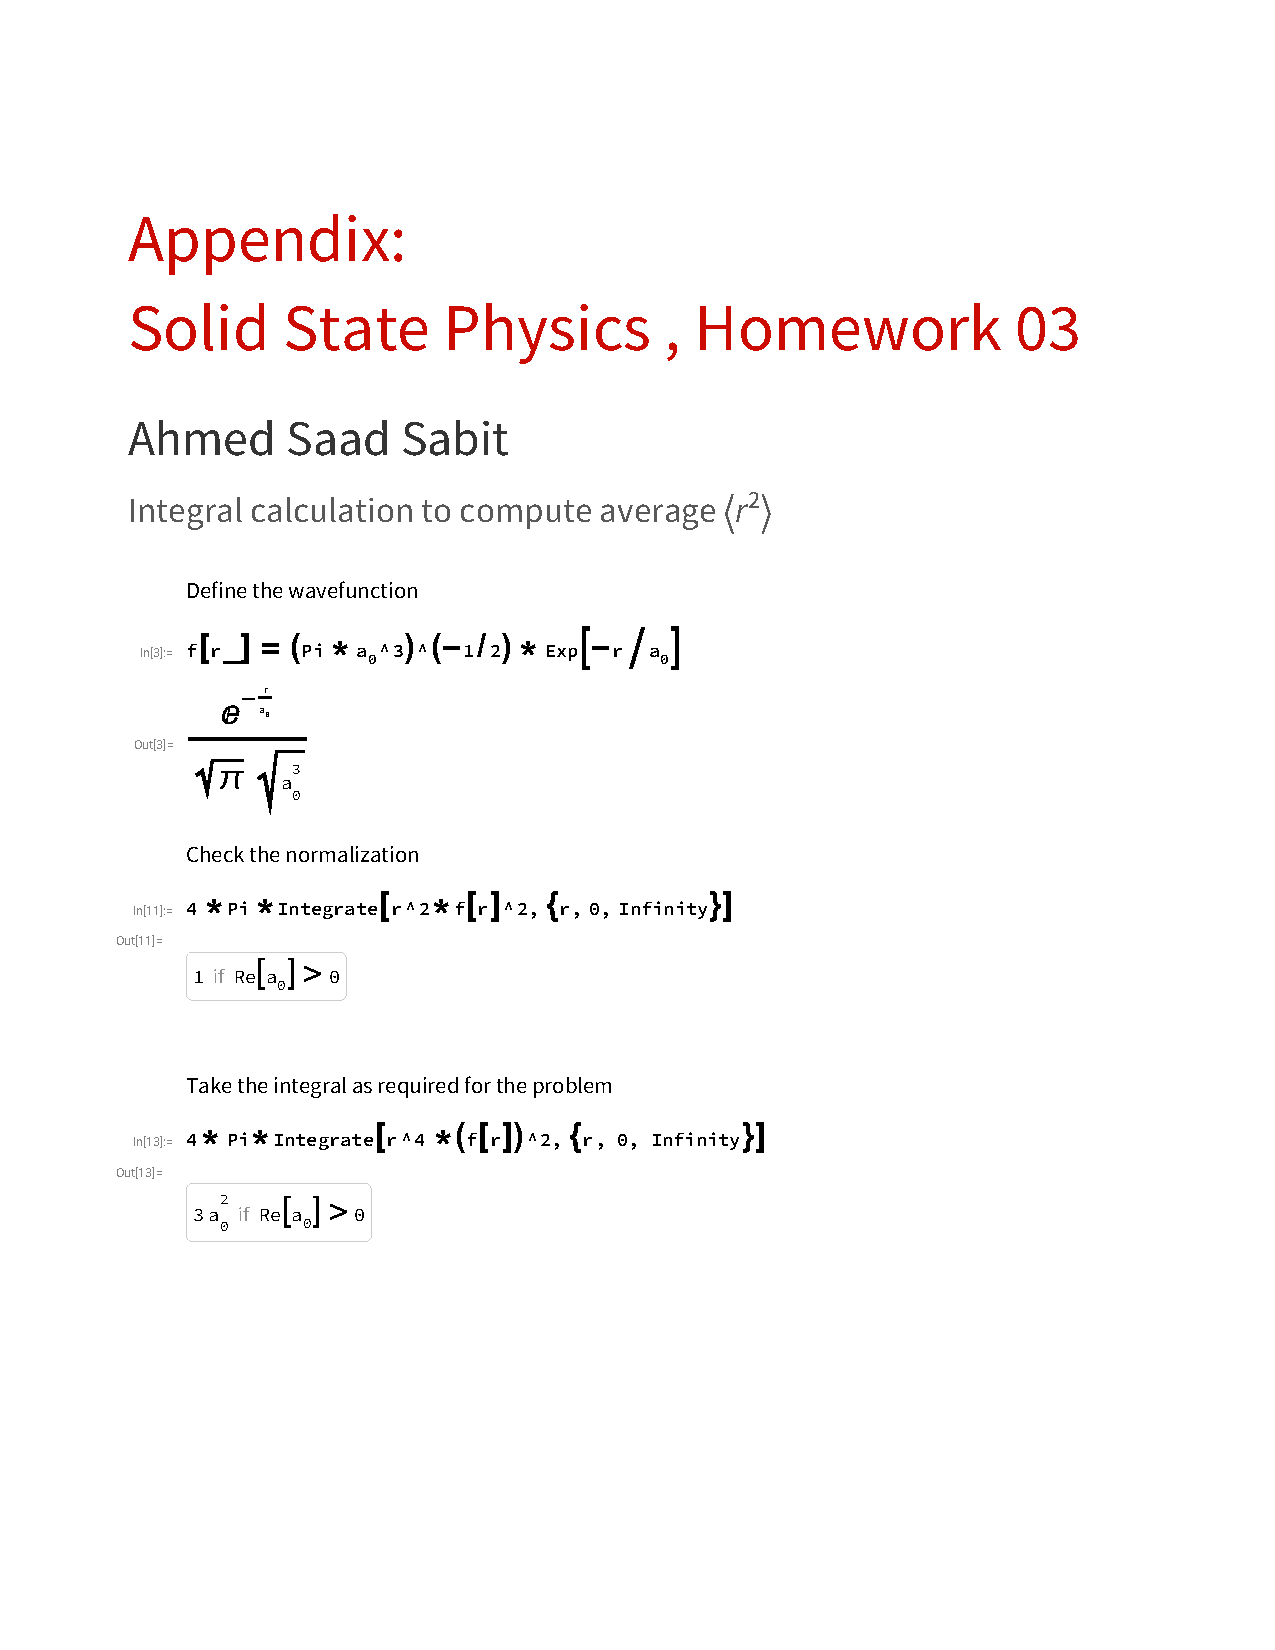
\includepdf[pages=-]{homework-3-appendix.pdf}
\end{document}
